% 24th, Jan, 2001 Ver.1     Tatsuya Okabe
%                 Ver.2
%                 Ver.3
%                 Ver.4
%                 Ver.5
%
%---------------------------------------------------------------------------%
% Made by Tatsuya Okabe ( HONDA R&D Europe ( Deutschland ) GmbH )           %
% Checked by Bernhard Sendhoff ( HONDA R&D Europe ( Deutschland ) GmbH )    %
%---------------------------------------------------------------------------%
% Class Normal

\section{Abstract}

\noindent
With the class {\em Normal}, the ``Normal'' or ``Gaussian''
distribution can be simulated. The corresponding equation is given below.

\begin{equation}
f(x) = \frac{1}{\sqrt{2\pi}\sigma} \cdot \exp{\frac{-(x-\mu)^2}{2\sigma^2}}
\end{equation}

\noindent
In this equation, $x$, $\sigma$ and $\mu$ mean the factor, the deviation
and the average, respectively.

\noindent
In this class, Box-Muller method was used to generate the random
numbers. Please refer [\ref{NRC}] to get more information.

%********************
\index{Box-Muller Method}
%********************

\vspace*{10mm}

\begin{center}
\begin{figure}[h]
\rotatebox{-90}{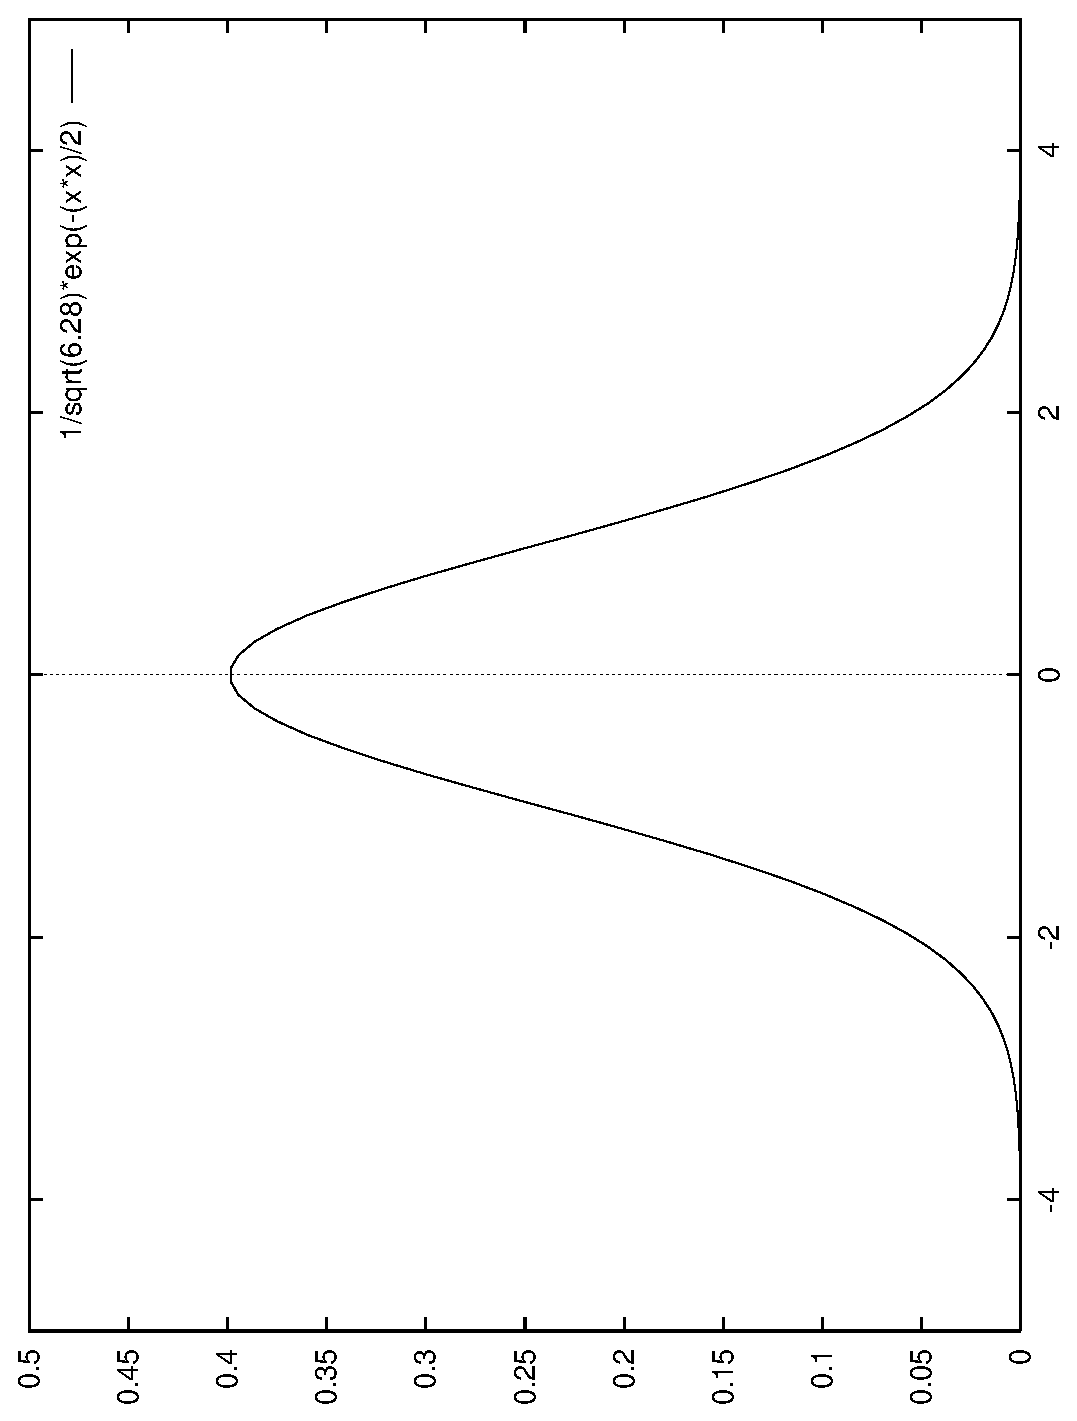
\includegraphics[height=12cm]{normal.eps}}\\
\caption{The Normal distribution. $\sigma=1$ and $\mu=0$.}
\end{figure}
\end{center}

\clearpage

\section{Internal Variables}

\begin{itemize}
\item pMean - The average.
\item pStdDev - The deviation.
\item iset - The flag in Box-Muller method ( existance of random
number ).
\item gset - The variable to store the random number.
\end{itemize}

%********************
\index{pMean (Variable)}
\index{pStdDev (Variable)}
\index{iset (Variable)}
\index{gset (Variable)}
%********************

\vspace*{10mm}

\section{Public Methods}

\noindent
These methods can be used by all \cpp - programs, that have included the
header file Normal.h and the library EA.

\subsection{Constructors}

%---------------------------------------------------------------------------%
% 001
\index{Normal!( double mean, double variance )}
\setNormalInstance
\setCorrectWidthThree{8pt}
\setParamOne{mean}{double}{The average.} 
\setParamTwo{variance}{double}{The variance.}
\printMethodWithParamsSaved
{}
{None.}
{Normal}
{The default constructor. Generates the random generator of Normal distribution.}
{None.}
\setCorrectWidthThree{4pt}
%---------------------------------------------------------------------------%

%---------------------------------------------------------------------------%
% 002
\index{Normal!( double mean, double variance, RNG\& rng )}
\setNormalInstance
\setCorrectWidthThree{8pt}
\setParamOne{mean}{double}{The average.} 
\setParamTwo{variance}{double}{The variance.}
\setParamThree{rng}{RNG\&}{RNG class.}
\printMethodWithParamsSaved
{}
{None.}
{Normal}
{The constructor. Generates the random generator of Normal distribution.}
{None.}
\setCorrectWidthThree{4pt}
%---------------------------------------------------------------------------%

\clearpage

\subsection{Operators}

%---------------------------------------------------------------------------%
% 003
\index{operator( )!( double mean, double variance )}
\setNormalInstance
\setCorrectWidthThree{8pt}
\setParamOne{mean}{double}{The average.} 
\setParamTwo{variance}{double}{The variance.}
\printMethodWithParamsSaved
{double}
{The result of normal distribution {\em N( mean, variance )}.}
{operator}
{Gets the result of normal distribution {\em N( mean, variance )}.}
{None.}
\setCorrectWidthThree{4pt}
%---------------------------------------------------------------------------%

%---------------------------------------------------------------------------%
% 004
\index{operator( )!( )} 
\setNormalInstance
\printEmptyMethodReturnSpecial
{double}
{operator( )}
{Gets the result of normal distribution {\em N( pMean, (pStdDev)$^2$ )}.}
{The result of normal distribution {\em N( pMean, (pStdDev)$^2$ )}.}
{None.}
%---------------------------------------------------------------------------%

\vspace*{10mm}

\subsection{Information Retrieval Methods}

%---------------------------------------------------------------------------%
% 005
\index{mean!( )} 
\setConstInstance
\printEmptyMethodReturnSpecial
{double}
{mean}
{Returns the average {\em pMean}.}
{The average {\em pMean}.}
{None.}
%---------------------------------------------------------------------------%

%---------------------------------------------------------------------------%
% 006
\index{variance!( )} 
\setConstInstance
\printEmptyMethodReturnSpecial
{double}
{variance}
{Returns the variance {\em (pStdDev)$^2$}.}
{The variance {\em (pStdDev)$^2$}.}
{None.}
%---------------------------------------------------------------------------%

\clearpage

%---------------------------------------------------------------------------%
% 007
\index{mean!( double newMean )} 
\setNormalInstance
\printMethodWithOneParam
{void}
{mean}
{double}
{newMean}
{New value of the average.}
{Sets the average {\em pMean} using new average {\em newMean}.}
{None.}
{None.}
%---------------------------------------------------------------------------%

%---------------------------------------------------------------------------%
% 008
\index{variance!( double newVar )} 
\setNormalInstance
\printMethodWithOneParam
{void}
{variance}
{double}
{newVar}
{New value of the variance.}
{Sets the deviation {\em pStdDev} using square root of new variance
{\em newVar}.}
{None.}
{None.}
%---------------------------------------------------------------------------%

\vspace*{10mm}

\subsection{Random seed}

%---------------------------------------------------------------------------%
% 009
\index{seed!( long s )} 
\setNormalInstance
\printMethodWithOneParam
{void}
{seed}
{long}
{s}
{Random seed.}
{Initializes the random seed.}
{None.}
{None.}
%---------------------------------------------------------------------------%

\vspace*{10mm}

\subsection{The probability}

%---------------------------------------------------------------------------%
% 010
\index{p!( const double\& x )} 
\setConstInstance
\printMethodWithOneParam
{double}
{p}
{const double\&}
{x}
{The factor which you want to calculate the probability.}
{Returns the probability of {\em x}.}
{The probability.}
{None.}
%---------------------------------------------------------------------------%













